%% This is an example first chapter.  You should put chapter/appendix that you
%% write into a separate file, and add a line \include{yourfilename} to
%% main.tex, where `yourfilename.tex' is the name of the chapter/appendix file.
%% You can process specific files by typing their names in at the 
%% \files=
%% prompt when you run the file main.tex through LaTeX.


\chapter{NEMS manufacturing methods}

In the previous chapter, the design of the DGSPR sensor was optimized with respect to operation \& manufacturing based on simulations of the sensor, and conversations with NEMS manufacturers. In this chapter, three methods of NEMS manufacturing will be explored and the final method will be chosen such that the production process costs less than $\sim$ \$ 5,000.00, can actually be completed within a reasonable time frame at the University of Toronto, and results in extremely smooth grating side-walls (which is imperative). 

The NEMS methods that will be explored in this chapter are UV Lithography (UVL), Electron Beam Lithography (EBI), and Nano-Imprinting (NI). Each method has it's own advantages and disadvantages. 

It is important to note that the actual design to be fabricated can either be the optimized design ($h$ = 2.0 $\mu m$, $\Lambda$ = 1000 $nm$, and $w$ = 300 $nm$), or its negative ($w$ = 700 $nm$) depending on the NEMS method used. 

\section{Lithography}

Lithography is by far one of the most common procedures in NEMS and relies on selectively removing parts of a `mask' to generate a pattern mold. One then simply transfers that pattern over from the mask to a `resist' (a material sensitive to a certain type of exposure) before developing the resist. Once the resist is developed, one may then etch the underlying substrate, consequently transferring the mask pattern over to the substrate. 

Within lithography there are two main variants: Electron beam lithography and Ultraviolet based Photo-lithography. They differ mainly in the type of exposure used to develop the resist (and in other subtler ways), but they do also share many common operations. 

\subsection{Deep UV Lithography (UVL)}

Also known as photo-lithography, UVL is one of the common methods used in the industry to generate micron \& sub-micron length patterns (or in engineering terms - in the order of a few hundredths of a thou to a few thou). The resolution of the pattern is limited by the light used to develop the resist, the dimensions of the photo-mask, the aperture of the optical lens system, and various other process-related factors. It is a good estimate (upper bound) to say that the `critical dimension' for the photo-lithography process is on the order of the wavelength of the light used \footnote{As an engineering rule of thumb one may use $\frac{\lambda}{2}$ as an estimate for the critical dimension.}. Thus for UVL, the resolution is around $\sim$ 150 to 200 $nm$ (using wavelength values for far UV and middle UV). 

The first step of the process is to make the photo-mask which contains the pattern which will be transferred onto the resist. It is theoretically possible to do mask-less UVL, using direct laser writing or maybe interference lithography, but these are limited in scope. Direct laser writing tends to have a large critical dimension (a few times larger than when using a mask), and interference lithography is limited to periodic patterns and truncated Fourier accuracy \footnote{If one were to Fourier transform a square wave and reconstruct it using only the first 7 harmonics of the sinusoidal reconstruction, the resultant square wave reconstruction would be significantly smoothed out. This is similar to what happens in interference lithography.}. 

The process of creating a mask (especially a simple periodic grating pattern) is best left to a commercial manufacturer - considering both the quality of the mask and the cost of making the mask - and will not be explained in detail. Such masks tend to cost around \$500 to \$1,000. To find such manufacturers one may consult \cite{mask_ind}. 

To get the substrate ready for processing, one must coat it with a photo-resist. This is usually something like SU8, ZEP, or PMMA. To coat the substrate one may spin coat it with the resist. The thickness of the resist layer is completely controlled by the RPM and run time of the spin-coating operation. Once the substrate has been coated with resist it should be pre-baked (or `cured') to get rid of excess.

Once the mask has been made (or bought), one must transfer the pattern over onto the photo-resist. This can be done by placing the mask on top of the resist, aligning it carefully with a mask-aligner, and then exposing the combination to light (usually UV). The resist will interact with the light and its molecular construction will change. After sufficient time exposing the resist to light, it can be `developed' to remove only the unexposed resist(or only the exposed - depends on if positive or negative resist), leaving behind the pattern that was originally on the mask. This is then baked to harden the remaining resist, making it a better protective layer for the etching process.

After the resist has been developed, the substrate is `etched'. There are multiple ways to do the etching process (e.g. wet etch or ion-etching) but the fundamental idea is the same. The etching process removes the layers of the substrate that are not protected by the developed resist. The run-time of the etch is usually what controls the depth of the etching process, though there can be other influencing factors such as the voltage in DRIE.

After the etching process, the remaining resist is removed and one is left with a patterned substrate. A more in-depth discussion of the photo-lithography process is available in \cite{UVL_intro}. 

\subsubsection{Issues with UVL}

The larger the design, the more applicable UVL becomes. For patterns with smaller dimensions (on the same scale as the exposure wavelength) we get artifacts generated during the exposure process \footnote{An example of such an artifact is side wall corrugation as explored in \cite{DeepUV}.}. These in turn lead to etching errors on the scale of ~10 to 20 $nm$. This is illustrated in \autoref{fig:bragg}, where it it obvious that the walls of the grating pattern exhibit side-wall corrugation. Such artifacts are frequent in UVL.

\begin{figure}
\centering
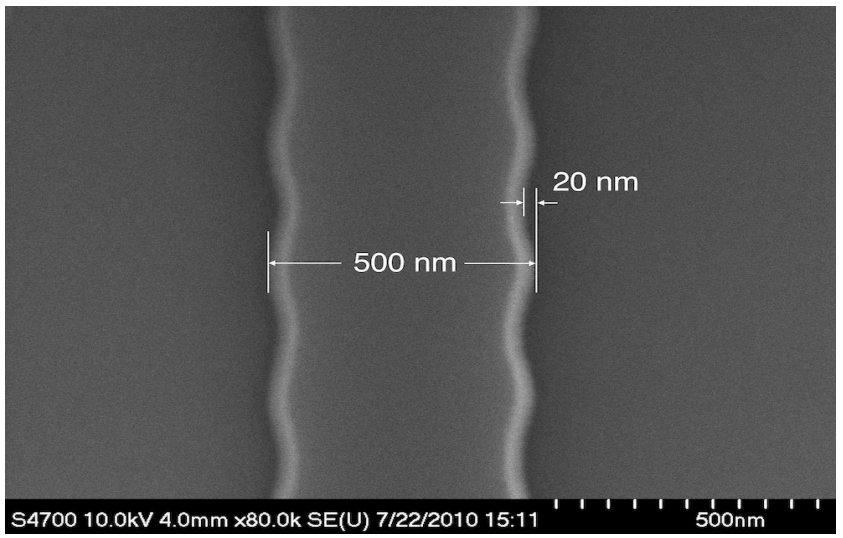
\includegraphics[width=0.75\textwidth]{bragg.png}
\caption{Figure showing an example of side-wall corrugation in Deep UVL. Image taken from \cite{DeepUV}}
\label{fig:bragg}
\end{figure}

Whilst UVL provides decent accuracy for sub-micron features, it comes into its own only for micron-scale features. Thus, for the purposes of manufacturing a DGSPR sensor, UVL does not satisfy the constraints. 

\subsection{Electron Beam Lithography (EBL)}

EBL shares much in common with UVL in that the method of developing the resist and etching are identical. The only real key change is that no mask is needed. The resist is placed on the substrate by spin-coating and is exposed directly to a moving electron beam which alters the resist's chemical makeup. The EBL method at the University of Toronto has a critical dimension of about 10 $nm$.

The electron-beam has an extremely small `write-field' which means that for large designs (anything over 25 $nm \times$ 25 $nm$), the design will be broken into smaller quadrilaterals and each quadrilateral will be exposed one after the other. 

After the design is exposed to the electron beam, the process of developing the resists and etching the substrate remains the same as with UVL. 

The EBL system at the University of Toronto costs about \$400 per hour.

\subsubsection{Issues with EBL}

It is important to note that there a few additional, unwanted phenomena that occur with EBL. One such phenomenon is the forward scattering of the electrons as they pass through the resist, combined with the backwards scattering of the electrons from the substrate. This scattering causes the degradation of the pattern during exposure (shown in \autoref{fig:scatter}). The degradation is due to the fact that any parts of the resist exposed to scattered electrons are also developed in conjunction with the intended pattern, thus causing significant variations. This degradation due to scattering can be modeled by a double Gaussian \cite{chang} (a sharp Gaussian to simulate forward scattering and a wide Gaussian to simulate back scattering) which is in turn called the proximity function. The degradation effect is hence called the `proximity effect'. 

\begin{figure}
\centering
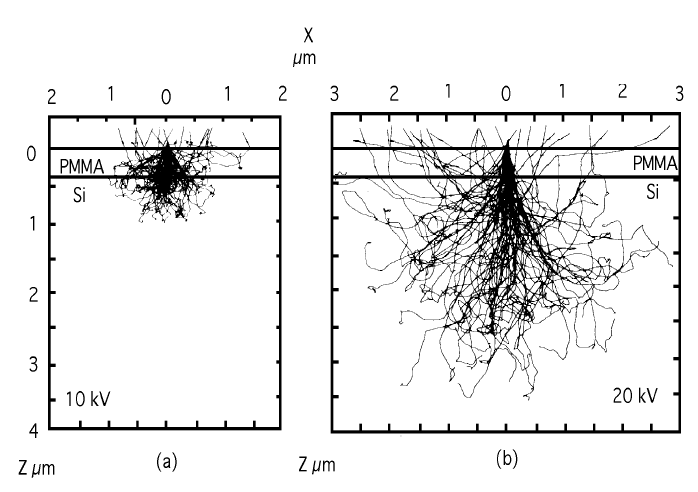
\includegraphics[width=0.75\textwidth]{scatter.png}
\caption{Figure showing an example of proximity effects in PMMA on Silicon. Image taken from \cite{kyser}.}
\label{fig:scatter}
\end{figure}

It is possible to correct for this using Proximity Effect Correction (PEC) by simulating proximity effects due to scattering before a design is exposed, and then altering the design dimensions or the exposure time/strength to counter the degradation. The PEC method and the algorithm used to reverse-engineer the effect are explained in \cite{PEC} to great detail. 

The University of Toronto recently invested in such a PEC system but no method is perfect and some degradation of the pattern should still be expected. 

Another unwanted phenomenon is that of stitching error. Due to the vector-scan writing implementation used by most EBL systems, the overall pattern is created by stitching together many smaller write-fields. This causes something known as the stitching error which arises from the misalignment of various write fields. This is illustrated best using \autoref{fig:stitching}. The typical stitching error value in the machine used by the University of Toronto is 25 $nm$. 

The effects of stitching error usually compound quickly and tend to cause extremely significant, somewhat local, discontinuities in the pattern (as in \autoref{fig:stitch_sig}). Even applying specialized methods to minimize the stitching error (as explained in \cite{stitch_signi}) and taking the utmost care and precaution when using EBL, we can still only reduce the effects of stitching error to about 10 $nm$ (which has the potential to quickly multiply). The realistically way to minimize the effects of stitching error is to make the written pattern as wide as possible. An error of 10 $nm$ on something that 1 $\mu m$ wide is a lot less significant than the same error on something thats 100 $nm$ wide.

\begin{figure}
\centering
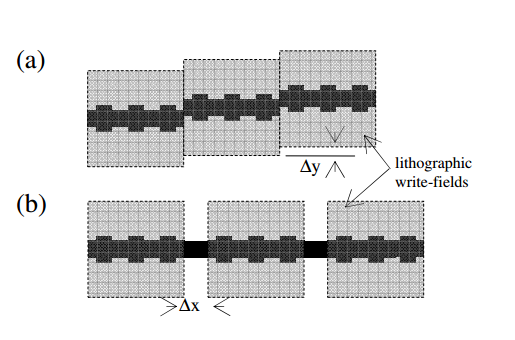
\includegraphics[width=0.75\textwidth]{stitching.png}
\caption{Figure showing a typical angle of both $x$ and $y$ stitching error. Image taken from \cite{stitch_img}.}
\label{fig:stitching}
\end{figure}

\begin{figure}
\centering
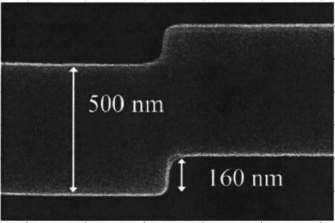
\includegraphics[width=0.75\textwidth]{w500nm_160nm.png}
\caption{Figure showing a significant stitching defect in a grating. Image taken from \cite{stitch_signi}.}
\label{fig:stitch_sig}
\end{figure}

The effect of all of these unwanted phenomena is that the walls of the exposed pattern, after developing \& etching, tend to be somewhat rough - which cannot be tolerated in the manufacturing of the DGSPR. 

\subsection{Nano-Imprinting (NI)}

NI is based on mechanically modifying a resist to imprint a pattern. That is, NI uses direct contact between a `master' mold and a resist to transfer a pattern from the master to the resist. Unlike with UVL or EBL, the process does not require any fancy equipment once the master has been made. It is cheap, easy to use. Furthermore, since NI uses direct contact, it overcomes the limitations set by light diffraction or beam scattering as in UVL or EBL. 

There are two main variants of NI: Hot Embossing or Thermal NI (TNI), and UV cured NI (UVNI). In TNI, the resist is spin coated onto the substrate. The master is pushed into the resist and left there under a certain pressure. The resist is simultaneously heated up above the glass transition temperature. The system is then cooled and the master is removed. In UVNI (shown in \autoref{fig:UVNI}), instead of heating up the resist, UV light is shined through a transparent master to cure the resist thus transferring the pattern. 

In both cases, once the pattern has been transferred the etching process can be started. 

\begin{figure}
\centering
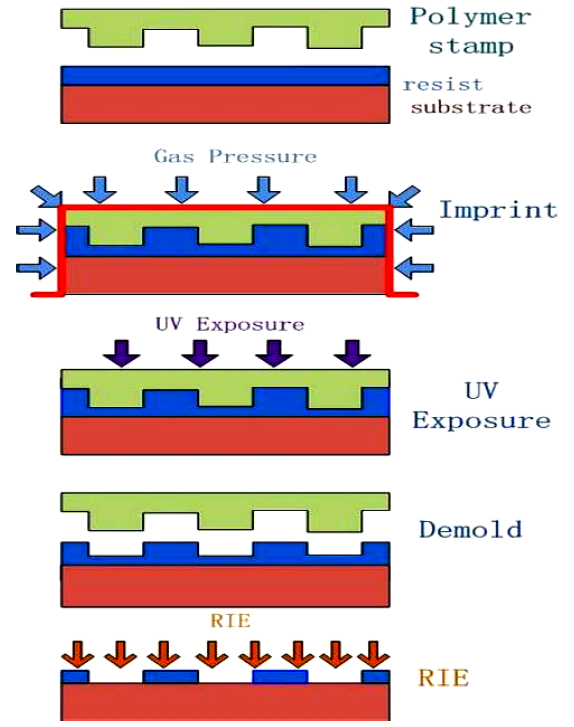
\includegraphics[width=0.75\textwidth]{UVNI.png}
\caption{Figure showing UVNI process. Image taken from \cite{UVNI_paper}.}
\label{fig:UVNI}
\end{figure}

The resolution and fabrication quality achievable by NI for $nm$ scale features far exceeds UVL. NI has similar resolution ($\sim$ 10 $nm$) to EBL but, assuming the master mold has no significant defects, the imprinted pattern using NI will be of a better quality than with EBL (due to it being a contact process). 

\section{Proposed Manufacturing Method}
After considering the constraints imposed at the beginning of this chapter - focusing mainly on the fact that the walls of the DGSPR's grating need to be smooth - NI was selected. Thus the problem of producing the gratings reduces mainly to the problem of making the corresponding master mold and as such, the identified constraints will be applied to the making of the master mold instead of the complete DGSPR structure. 

The method used to make the master mold is a combination of EBL, DRIE and wet-etching (if required). The selected method is a variant of a method described in the paper written by Yu et al. \cite{sexy_des_method} and should result in a grating structure with extremely smooth side-walls.  

Yu's method is aimed at creating a master mold for a grating structure in Silicon, using the inbuilt geometry of the Silicon crystal (i.e. using the fact that the crystal planes are practically perfectly straight). A (110) Silicon substrate is used as the mold surface and a layer of thick oxide is grown. The gratings are carefully aligned to the \{111\} reference flat of the Silicon crystal and etched using an Argon-Ion laser onto the thick $SiO_2$ layer. The pattern is then transferred from the $SiO_2$ layer, onto the Silicon (110) substrate using DRIE. If the walls are insufficiently smooth then a KOH wet-etch may be applied. Since the KOH wet-etch is extremely anisotropic (i.e. extremely slow in the $\langle 111 \rangle$ direction) this will result in extremely smooth side-walls. The entire process is explained in greater detail in \cite{sexy_des_method}. The master mold created using this method, can then be used in the imprinting of other resists. Since the master has extremely smooth side-walls, so too do the imprinted resists. An example of a mold so created is visible in \autoref{fig:Yu_mold}, and an example of an imprinted resist is visible in \autoref{fig:Yu_res}.

\begin{figure}
\centering
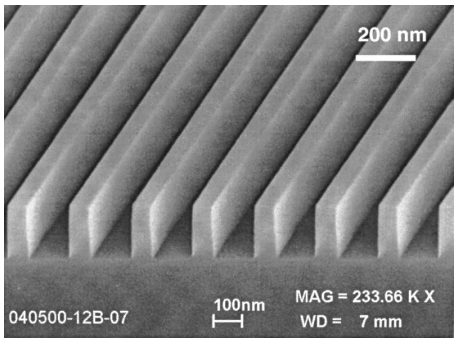
\includegraphics[width=0.75\textwidth]{Yu_mold.png}
\caption{Figure showing smooth mold side-walls created using Yu's method. Image taken from \cite{sexy_des_method}.}
\label{fig:Yu_mold}
\end{figure}

\begin{figure}
\centering
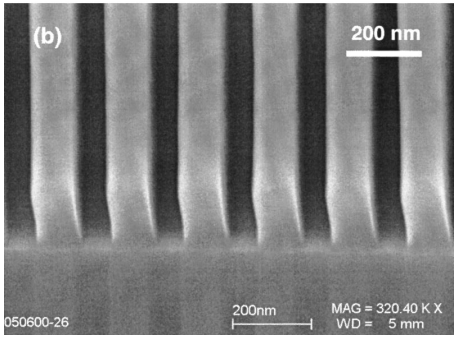
\includegraphics[width=0.75\textwidth]{Yu_res.png}
\caption{Figure showing smooth side-walls in imprinted resist using a mold created using Yu's method. Image taken from \cite{sexy_des_method}.}
\label{fig:Yu_res}
\end{figure}

The variation on this method is to use EBL with negative resist to generate the grating pattern on top of the Silicon substrate. Once the grating pattern is generated, the etching of the Silicon master can be done using DRIE etching \footnote{Theoretically, a Pseudo Bosch etching process should allow for extremely smooth nano-scale etching, making the KOH wet-etch step unnecessary.}. To smooth out any rough side-walls, a KOH wet-etch will be applied post DRIE (if required). This method will henceforth be known as the `smooth wall etching process' or `wall-e' for short. %`modified etching process' or ‘mod-e' for short.

\section{Summary}

In this chapter an overview of the three main NEMS manufacturing methods was provided and a method to actually fabricate a master mold (which will be used in turn to fabricate a DGSPR sensor using NI) was selected.  
